\documentclass[a4paper, 12pt]{article}%тип документа

%отступы
\usepackage[left=2cm,right=2cm,top=2cm,bottom=3cm,bindingoffset=0cm]{geometry}

%Русский язык
\usepackage[T2A]{fontenc} %кодировка
\usepackage[utf8]{inputenc} %кодировка исходного кода
\usepackage[english,russian]{babel} %локализация и переносы

%Вставка картинок
\usepackage{wrapfig}
\usepackage{graphicx}
\graphicspath{{pictures/}}
\DeclareGraphicsExtensions{.pdf,.png,.jpg}

%оглавление
\usepackage{titlesec}
\titlespacing{\chapter}{0pt}{-30pt}{12pt}
\titlespacing{\section}{\parindent}{5mm}{5mm}
\titlespacing{\subsection}{\parindent}{5mm}{5mm}
\usepackage{setspace}

%Графики
\usepackage{multirow}
\usepackage{pgfplots}
\pgfplotsset{compat=1.9}

%Математика
\usepackage{amsmath, amsfonts, amssymb, amsthm, mathtools}

%Заголовок
\author{Валеев Рауф Раушанович \\
группа 825}
\title{\textbf{Работа 3.2.4\\Свободные колебания в электрическом контуре}}
\newtheorem{task}{Задача}
\date{}
\begin{document}
\maketitle
\newpage
\section*{Цель работы}
Исследование свободных колебаний в электрическом контуре.
\section*{В работе используются}
Генератор импульсов, электронное реле, магазин сопротивлений, магазин емкостей, катушка индуктивности, электронный осциллограф, универсальный измерительный мост. 
\section*{Теория}
\subsection*{Свободные колебания}
Рассмотрим электрический контур, состоящий из последовательно соединённых конденстора $C$, катушки индуктивности $L$ и резистора $R$. Обозначим разность потенциалов на конденсаторе $U_C$, а ток, текущий в контуре, через $I$. Второе првило Кирхгофа:
\begin{equation}
L \dfrac{d^2I}{dt^2}+R\dfrac{dI}{dt}+\dfrac{I}{C}=0.
\end{equation}
Вводя обозначения $\gamma = \dfrac{R}{2L}$, $\omega_0^2=\dfrac{1}{LC}$, получим уравнение
\begin{equation}
\ddot{I}+2\gamma\dot{I}+\omega_0^2I=0.
\end{equation}
Его решение в общем виде:
\begin{equation}
I = -\dfrac{U_0}{L\kappa}e^{-\gamma t}\text{sh}(\kappa t), 
\end{equation}
где $\kappa = \sqrt{\gamma^2 - \omega_0^2}$, $U_0 = U_C$ -- начальное напряжение на конденсаторе.

\subsection*{Затухающие колебания}
 В случае, когда $\gamma < \omega_0$, имеем $\kappa = i\omega$, где $\omega = \sqrt{\omega_0^2 - \gamma^2}$ -- \textit{частоты свободных (собственных) колебаний}. Тогда ток
 \begin{equation}
 I = -\dfrac{U_0}{L\omega}e^{-\gamma t}\sin(\omega t)
 \end{equation}
 затухает и имеет колебательный характер. Величина $\gamma$ определяет затухание колебаний: $\gamma = \dfrac{1}{\tau}$, где $\tau$ -- время затухание амплитуды в $e$ раз.
Формулы для наряжение на кондесаторе и тока в цепи можно переписать иначе:
\begin{equation}
\begin{array}{c}
U_C = U_0 \dfrac{\omega_0}{\omega}e^{-\gamma t} \cos(\omega t - \theta),\\
\\
I = -\dfrac{U_0}{L}e^{-\gamma t} \cos(\omega t - \theta).
\end{array}
\end{equation}
\subsection*{Апериодические колебания}
В случае $\gamma > \omega_0$, формулы для тока и напряжения на конденсаторе имеют следующий вид:
$$
\begin{array}{c}
I = -\dfrac{U_0}{L\kappa}e^{-\gamma t}\text{sh}(\kappa t),\\
\\
U_C = U_0 e^{-\gamma t}\left( \dfrac{\gamma}{\kappa}\text{sh}(\kappa t) + \text{ch}(\kappa t) \right).
\end{array}
$$
Процесс в этом случае не является колебательным, его называют апериодическим. Режим, соответствующий $\gamma = \omega_0$, называются \textit{критическим}. В этом случае предельный переход $\omega \rightarrow 0$ в $(5)$ даст 
$$
\begin{array}{c}
I = -\dfrac{U_0}{L}te^{-\gamma t},\\
\\
U_C=U_0 e^{-\gamma t}(1+\gamma t).
\end{array}
$$
Сопротивление в этом случае 
\begin{equation}
R_{\text{кр}}= 2 \sqrt{\dfrac{L}{C}}
\end{equation}
называется \textit{критическим сопротивлением} контура.\\
\textit{Добротность} контура по определению 
$$
Q = 2\pi \dfrac{W}{\Delta W},
$$ 
где $W$ -- запасённая энергия, $\Delta W$ -- потери за период. Тогда
$$
Q = 2\pi\dfrac{CU_0^2/2 \cdot e^{-2\gamma t}}{CU_0^2/2 \cdot (e^{-2\gamma t} - e^{-2\gamma (T+t)})}=\dfrac{\pi}{\gamma T}=\dfrac{1}{R}\sqrt{\dfrac{L}{C}}.
$$
\textit{Логарифмическим декрементом затухания} называются число
$$
\Theta = \text{ln}\dfrac{U_k}{U_{k+1}}=\text{ln} e^{\gamma T}=\gamma T
$$
или 
$$
\Theta = \dfrac{1}{n} \text{ln}\dfrac{U_k}{U_{k+n}}.
$$
\newpage
\section*{Установка}
\begin{figure}[h!]
\begin{center}
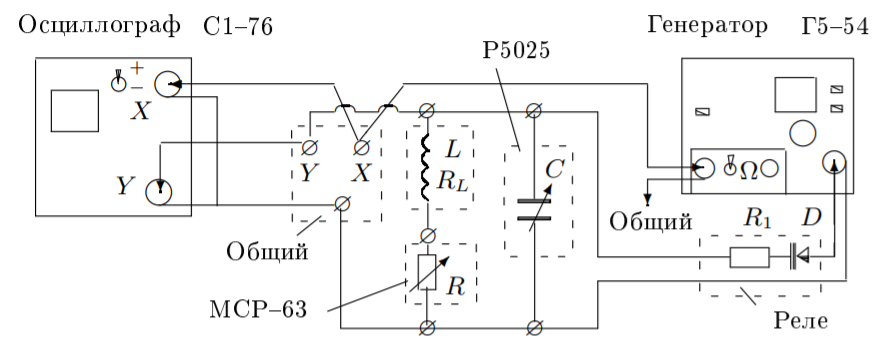
\includegraphics[width = 0.7\textwidth]{1.png}
\caption{Схема установки}
\end{center}
\end{figure}
На рисунке приведена схема для исследования свободных колебаний в контуре, содержащем постоянную индуктивность $L$ и переменные ёмкость $C$ и сопротивление $R$. Колебания наблюдаются на экране осциллографа.

Для периодического возбуждения колебаний в контуре используется генератор импульсов Г5-54. С выхода генератора по коаксиальному кабелю импульсы поступают на колебательный контур через электронное реле, смонтированное в отдельном блоке (или на выходе генератора). Реле содержит тиристор $D$ и ограничительный резистор $R_1$.

Импульсы заряжают конденсатор $C$. После каждого импульса генератор отключается от колебательного контура, и в контуре возникают свободные затухающие колебания. Входное сопротивление осциллографа велико ($\approx 1$ МОм), так что его влиянием на контур можно пренебречь. Для получения устойчивой картины затухающих колебаний используется режим ждущей развёртки с синхронизацией внешними импульсами, поступающими с выхода <<синхроимпульсы>> генератора.
\section*{Ход работы}
Прежде всего измерим индуктивность $L$ и сопротивление катушки $R_L$ в зависимости от частоты 

\begin{table}[h!]
\begin{center}

\begin{tabular}{|c|c|c|}
\hline
$\nu$, Гц & $L$, мГн & $R_L$, Ом \\ \hline
50        & 200,4    & 11,1      \\ \hline
1000      & 200,1    & 18,8      \\ \hline
5000      & 200,4    & 41,2      \\ \hline
\end{tabular}
\caption{Некоторые параметры катушки индуктивности}
\end{center}
\end{table}
В итоге мы получаем, что $L = 200 \pm 0,2$ мГн.
\newpage
\subsection*{Измерение периодов свободных колебаний}
Установим на магазине сопротивлений $R = 0$ Ом и $C = 0,02$ мкФ. Подобрав частоту развертки получим изображение наших колебаний на осциллографе. Из этого убедимся, что частота повторений, которую мы установили на генераторе ($\nu_0 = 100$ Гц) будет равна частоте повторения импульсов. 

\begin{figure}[h!]
\begin{center}
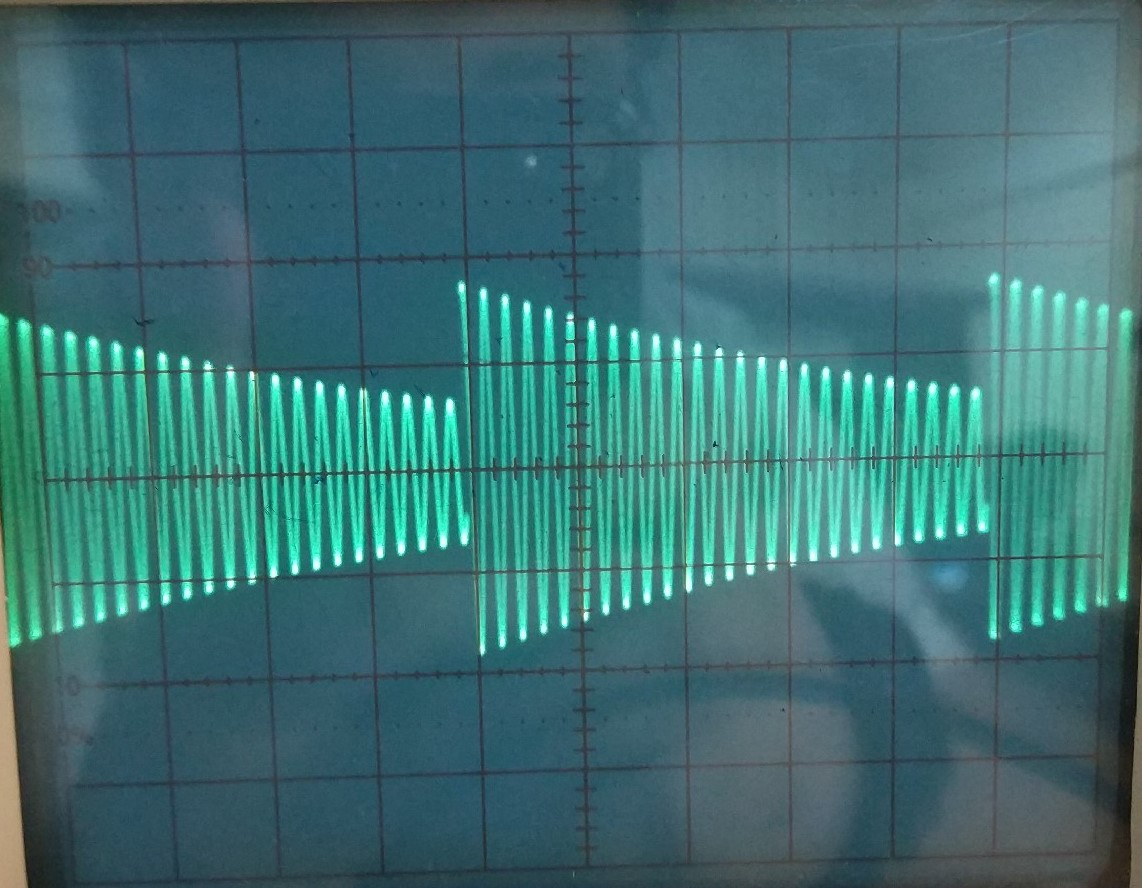
\includegraphics[width = 0.55\textwidth]{3.jpg}
\caption{Колебания в контуре}
\end{center}
\end{figure}

Теперь изменяя ёмкость в диапазоне $0,02 - 0,09$ мкФ проведем измерения периодов свободных колебаний и сравним их с теоретическими данными по формуле 
\[T = 2 \pi \sqrt{LC}\]

\begin{table}[h!]
\begin{center}
\begin{tabular}{|c|c|c|c|c|c|c|}
\hline
С, нФ & t, мс & $\sigma_t$, мс & $N$ периодов & $T_{prac}$, мс & $T_{theor}$, мс & $\sigma_T$, мс \\ \hline
20    & 5,0   & 0,3            & 12           & 0,42           & 0,40            & 0,03           \\ \hline
25    & 5,0   & 0,3            & 11           & 0,45           & 0,44            & 0,03           \\ \hline
30    & 5,0   & 0,3            & 10           & 0,50           & 0,49            & 0,03           \\ \hline
35    & 5,0   & 0,3            & 9,25         & 0,54           & 0,53            & 0,03           \\ \hline
40    & 5,0   & 0,3            & 8,75         & 0,57           & 0,56            & 0,03           \\ \hline
45    & 5,0   & 0,3            & 8,25         & 0,61           & 0,60            & 0,04           \\ \hline
50    & 5,0   & 0,3            & 7,75         & 0,65           & 0,63            & 0,04           \\ \hline
55    & 5,0   & 0,3            & 7,5          & 0,67           & 0,66            & 0,04           \\ \hline
60    & 5,0   & 0,3            & 7,25         & 0,69           & 0,69            & 0,04           \\ \hline
70    & 5,0   & 0,3            & 6,5          & 0,77           & 0,74            & 0,05           \\ \hline
\end{tabular}
\caption{Таблица данных измерения периода свободных колебаний и сравнение с теорией}
\end{center}
\end{table}

Видим, что теория очень хорошо сходится с экспериментом.
\section*{Измерение критического сопротивления и декремента затухания}
Для начала рассчитаем емкость, при которой частота собственных колебаний контура будет равна $\nu_0 = 5$ кГц.
\[C = \dfrac{1}{4 \pi^2 \nu_0^2 L} \approx 5 \text{нФ}\]
И для значений $L$ и $C$ рассчитаем $R_{crit}$
\[R_{crit} = 2\pi\sqrt{\dfrac{L}{C}} \approx 12,6 \text{кОм}\]
Для этих значений $L$ и $C$ рассчитаем декремент затухания для каждого сопротивления из интервала $(0,1-0,3)R_{crit}$. Из этих данных по формуле 
\[R_{crit} = R_{\Sigma} \sqrt{\left[\dfrac{2\pi}{\theta}\right]^2 + 1}\]
находим $R_{crit}$ запишем все в таблицу. 

\begin{table}[h!]
\begin{center}
\begin{tabular}{|c|c|c|c|c|c|c|c|c|}
\hline
R, Ом & $U_1$, дел & $\sigma_{U_1}$, дел & $U_2$, дел & $\sigma_{U_2}$, дел & $\theta$ & $\sigma_{\theta}$ & $R_{crit}$, Ом & $\sigma_{R_{crit}}$, Ом \\ \hline
1200  & 4          & 0,2                 & 2,1        & 0,2                 & 0,64     & 0,07              & 11800          & 1000                    \\ \hline
1500  & 4          & 0,2                 & 1,8        & 0,2                 & 0,80     & 0,10              & 11900          & 1300                    \\ \hline
1800  & 4          & 0,2                 & 1,6        & 0,2                 & 0,92     & 0,12              & 12500          & 1600                    \\ \hline
2100  & 4          & 0,2                 & 1,3        & 0,2                 & 1,1      & 0,2               & 11900          & 1400                    \\ \hline
2400  & 4          & 0,2                 & 1,1        & 0,2                 & 1,3      & 0,2               & 11900          & 1300                    \\ \hline
2700  & 4          & 0,2                 & 1          & 0,2                 & 1,4      & 0,3               & 12500          & 1000                    \\ \hline
3000  & 4          & 0,2                 & 0,8        & 0,2                 & 1,6      & 0,4               & 12000          & 1300                    \\ \hline
3300  & 4          & 0,2                 & 0,7        & 0,2                 & 1,7      & 0,5               & 12300          & 1600                    \\ \hline
\end{tabular}
\caption{Таблица измерения $R_{crit}$}
\end{center}
\end{table}

В итоге мы получаем, что $R_{crit} = (12,1 \pm 1,8)$ кОм.

Так же мы можем получить $R_{crit}$ просто подбором, добиваясь подобной картины

\begin{figure}[h]
\begin{center}
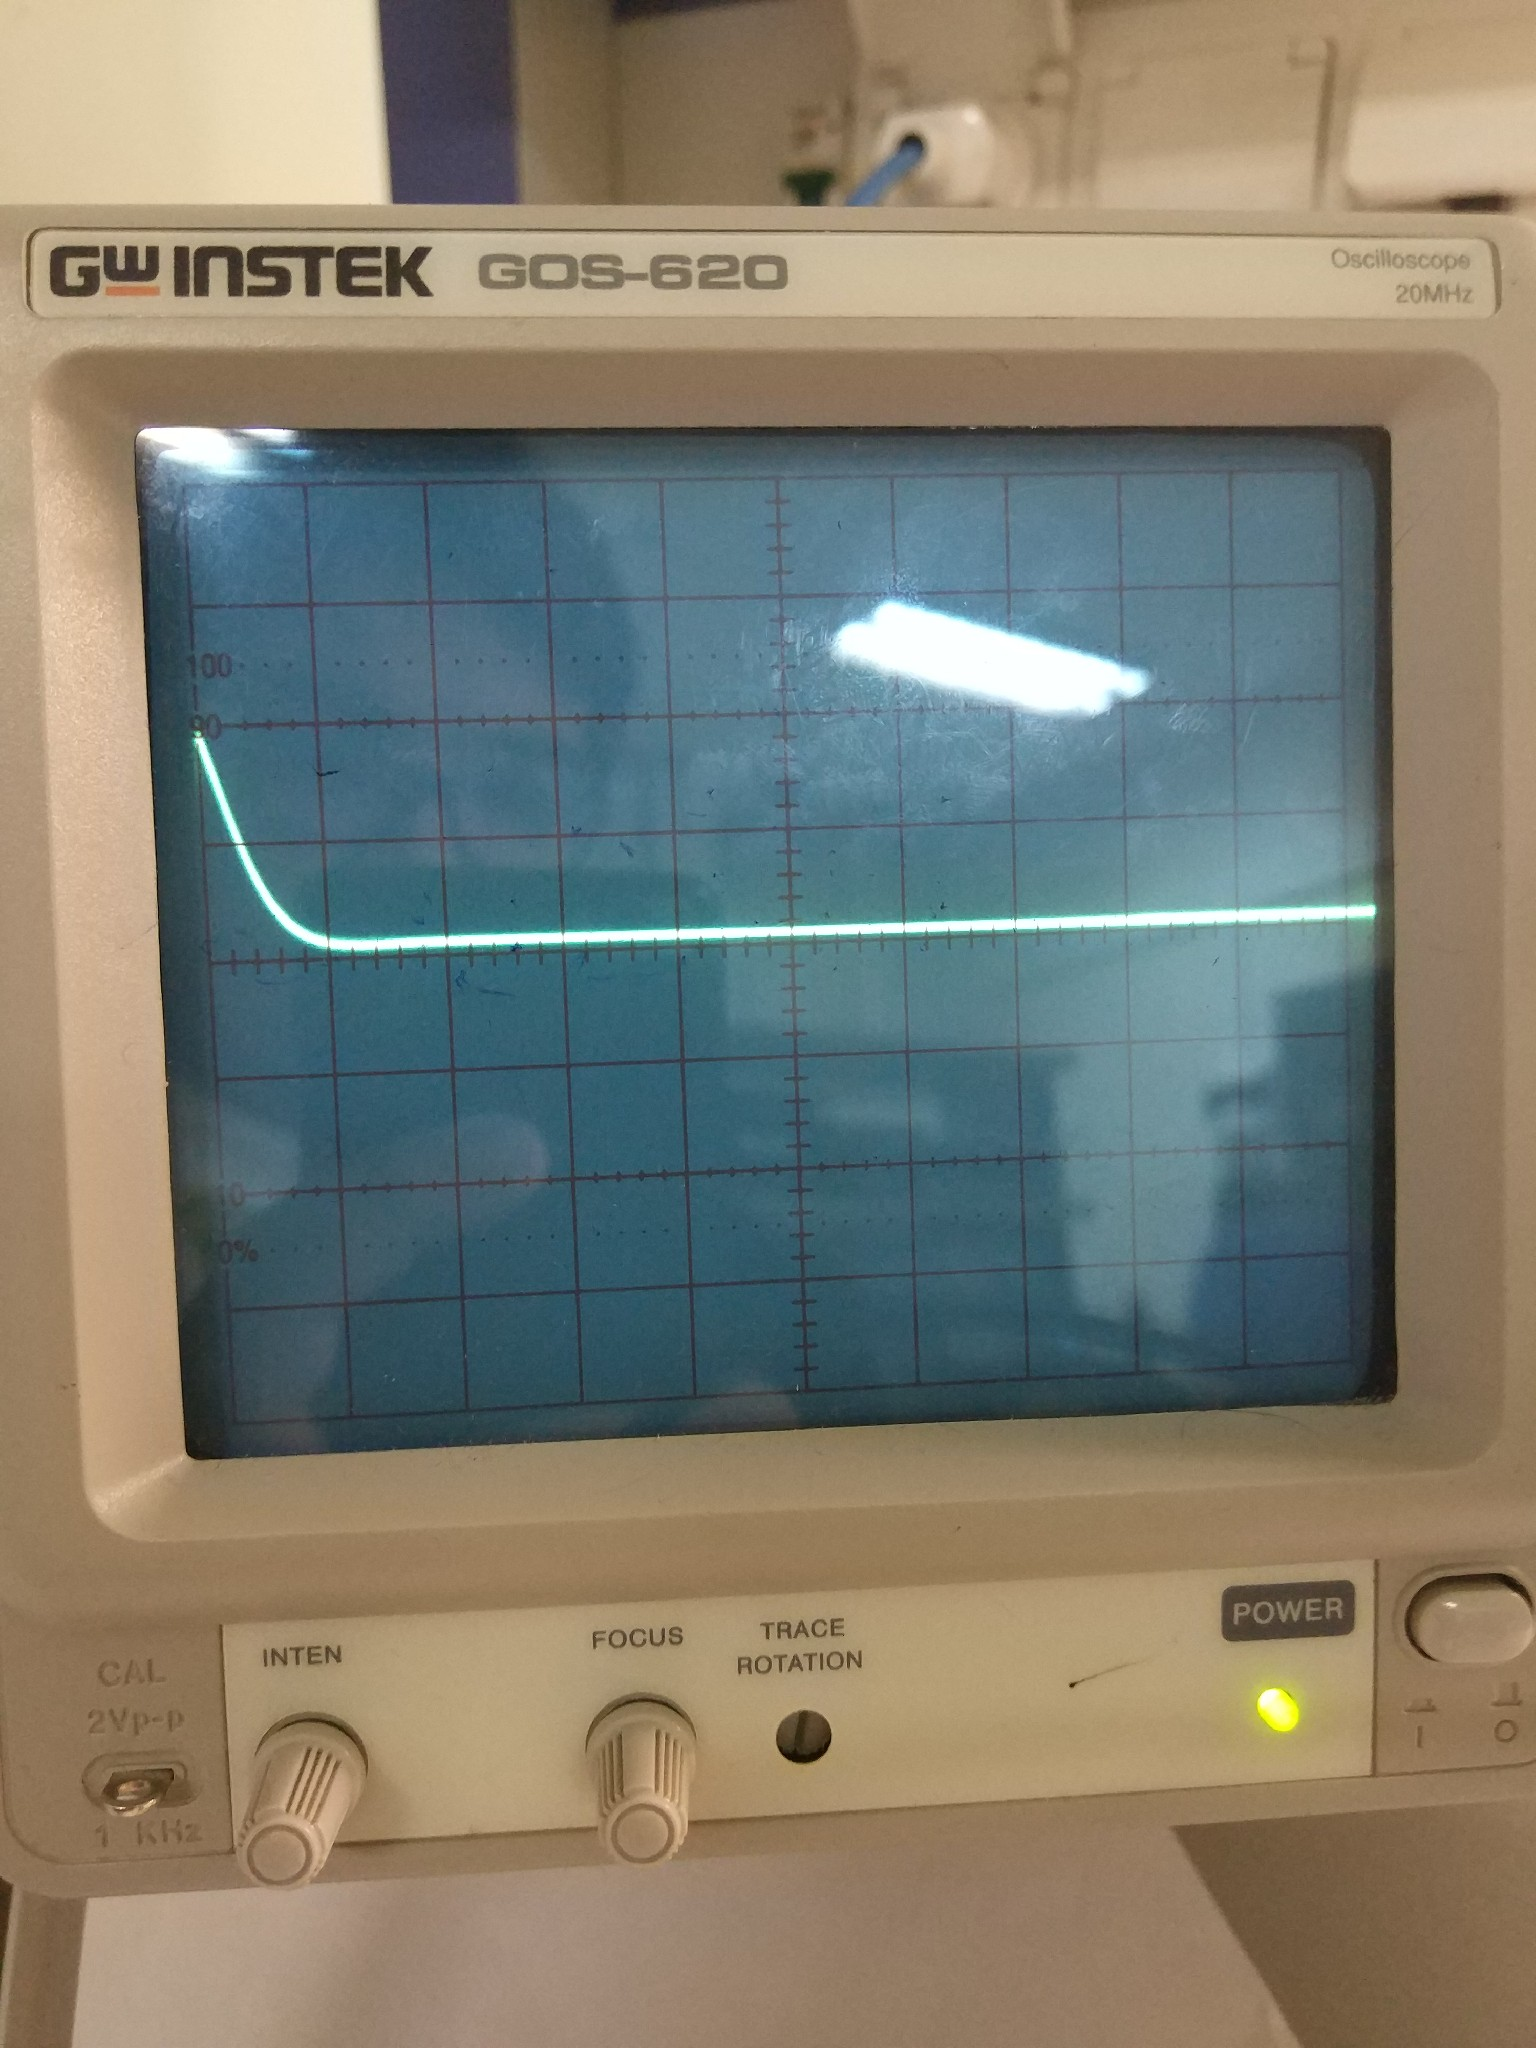
\includegraphics[width = 0.2\textwidth]{2.jpg}
\caption{Затухание колебаний}
\end{center}
\end{figure}

Подбирая мы получаем, что $R_{crit} \approx 12$ кОм.
\newpage
\subsection*{Свободные колебания на фазовой плоскости}
Рассмотрим свободные колебания на фазовой плоскости, для этого подключим место соединения катушки индуктивности и магазина сопротивлений к выходу $X$ и включим на осциллографе канал $X-Y$. В итоге мы получаем картинку на экране как на рисунке ниже. 
\begin{figure}[h!]
\begin{center}
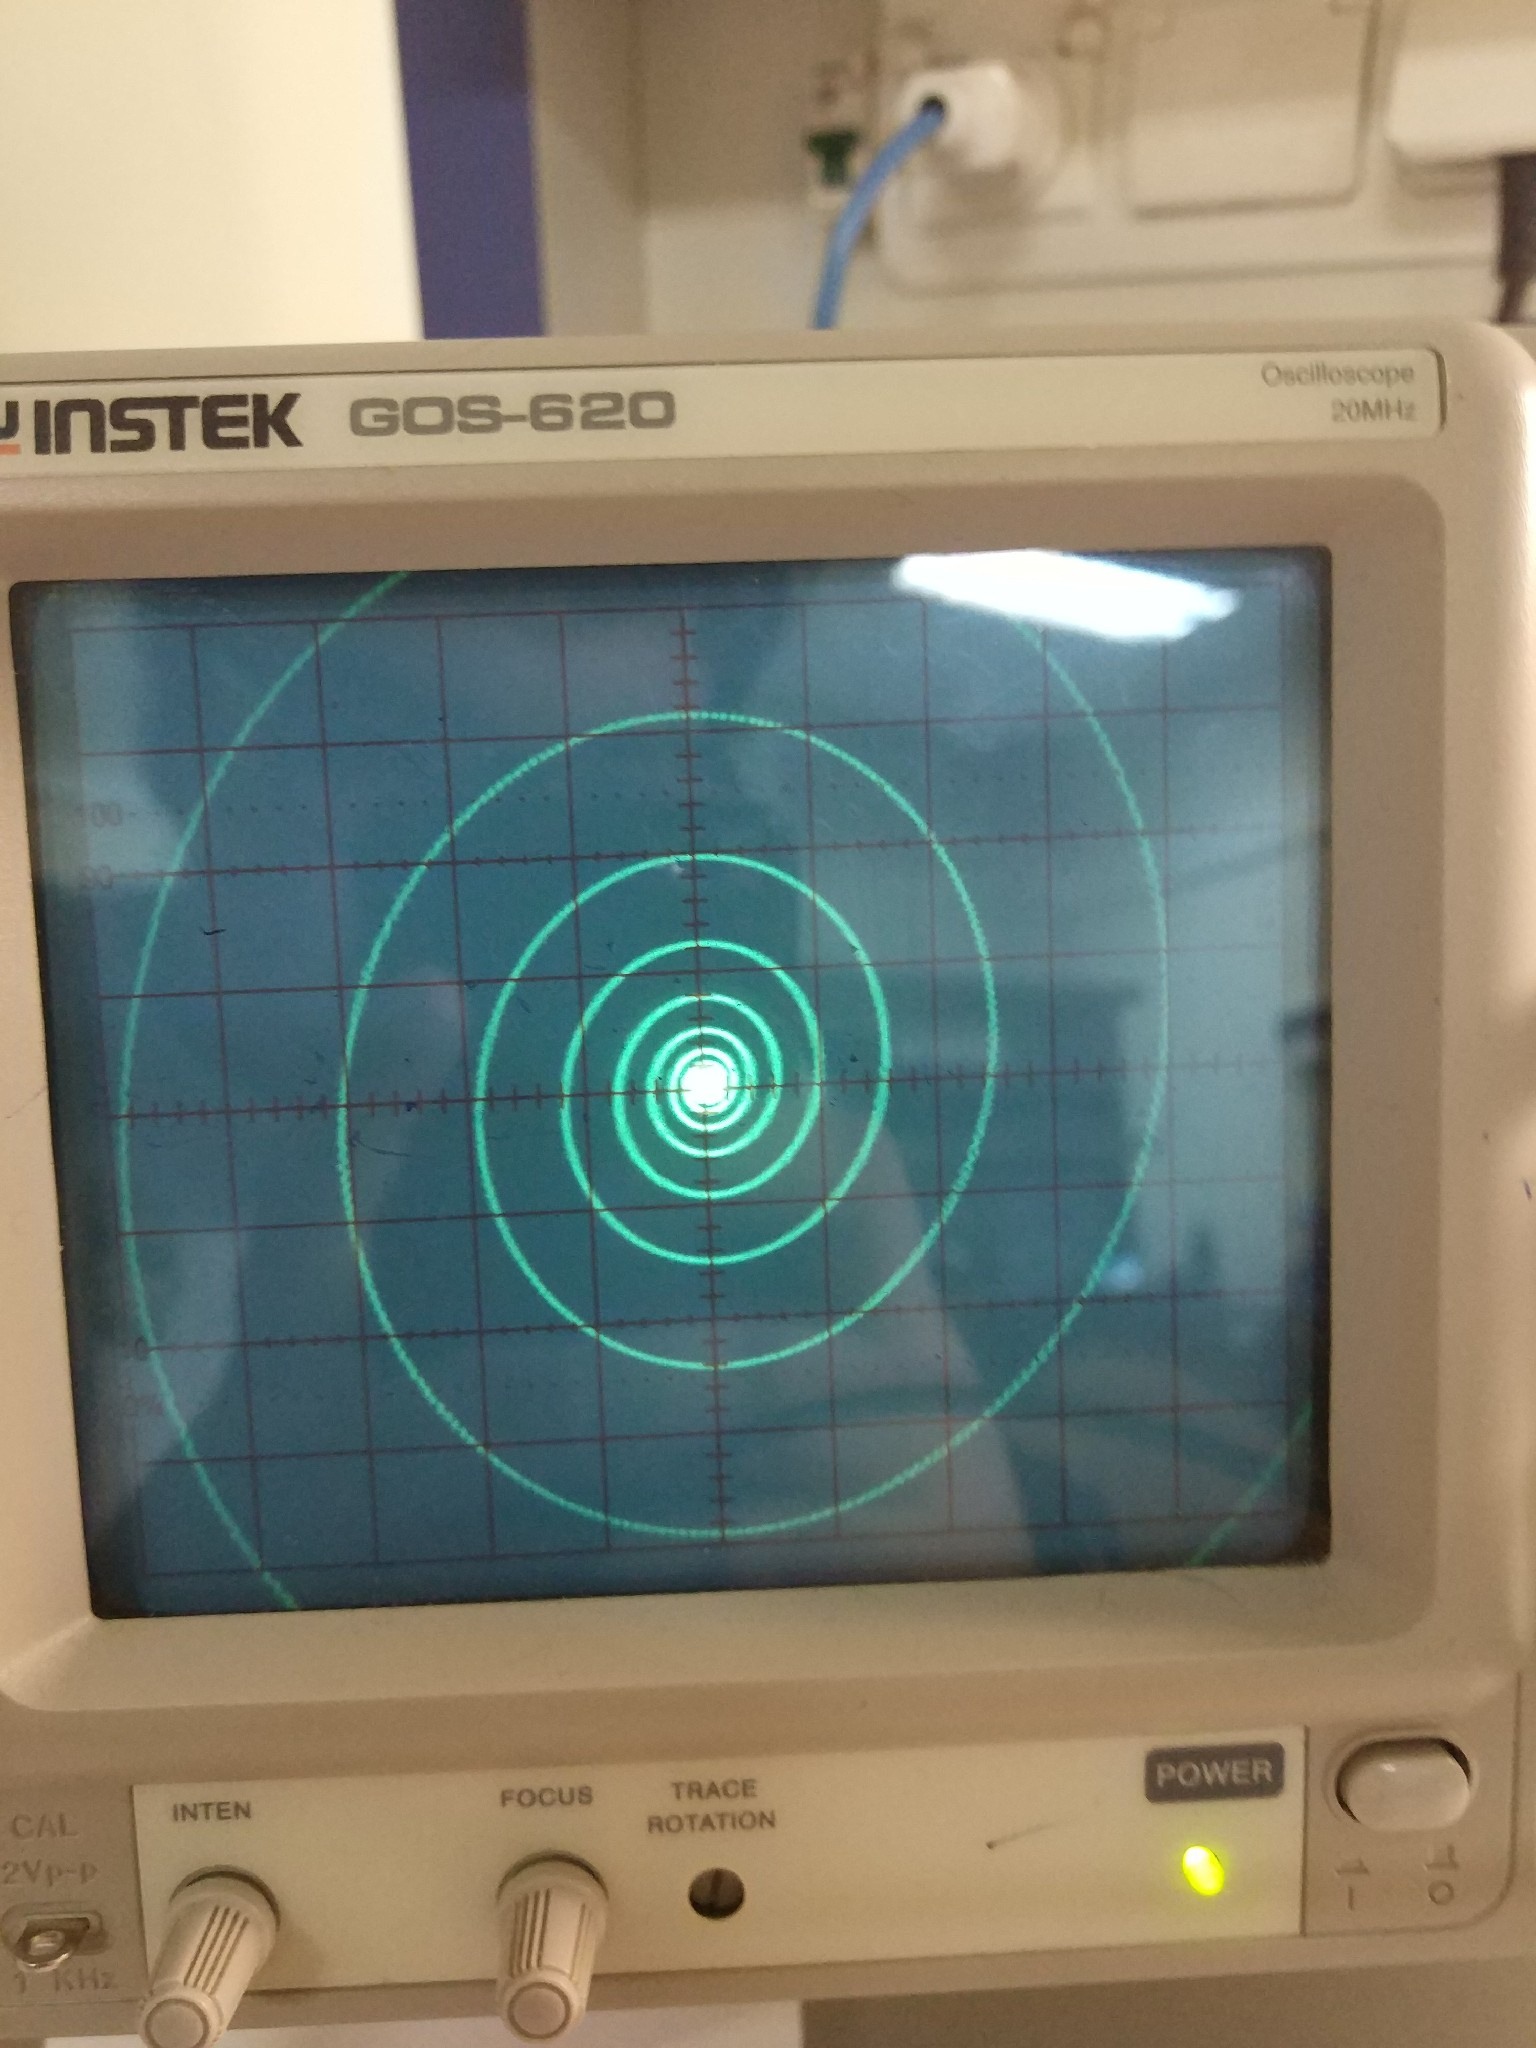
\includegraphics[width = 0.6\textwidth]{1.jpg}
\caption{Фазовая диаграмма для свободных колебаний}
\end{center}
\end{figure}

Для фазовой диаграммы для двух значений посчитаем так же декремент затухания

\begin{table}[h!]
\begin{center}
\begin{tabular}{|c|c|c|c|c|}
\hline
$R$, Ом &$U_1$, дел & $U_2$, дел & $\theta$ & $\sigma_{\theta}$ \\ \hline
1800 &4,1        & 1,6        & 0,94    & 0,15              \\ \hline
3000& 3          & 0,5        & 1,8     & 0,2              \\ \hline
\end{tabular}
\caption{Декремент затухания для фазовой диаграммы}
\end{center}
\end{table}

Видим, что мы получили такой же декремент затухания как и при его подсчете из графика колебаний.
\subsection*{Добротность свободных колебаний в контуре}
Добротность можно найти по формуле 
\[Q = \dfrac{\pi}{\theta}\]
Найдем ее для $R_{max} = 3$ кОм и для $R_{min} = 1,8$ кОм из графика и фазовой диаграммы. Итоговые результаты запишем в таблицу.

Так же добротность можно найти и из теоретических соображений по формуле
\[Q = \dfrac{1}{R}\sqrt{\dfrac{L}{C}}\]

Результаты так же занесем в таблицу, и в итоге мы получаем эту таблицу со всеми данными из данного эксперимента, по которой мы можем сравнить все полученные значения

\begin{table}[h!]
\begin{center}
\begin{tabular}{|c|c|c|c|c|c|c|c|}
\hline
\multirow{2}{*}{} & \multirow{2}{*}{$L_{coil}$, мГн} & \multicolumn{3}{c|}{$R_{crit}$, кОм}                         & \multicolumn{3}{c|}{Q}                 \\ \cline{3-8} 
                  &                                  & Теор.                 & Подбор              & Граф.          & Теор. & Граф.         & Спираль        \\ \hline
$R_{max}$         & \multirow{2}{*}{$200 \pm 0,2$}   & \multirow{2}{*}{12,6} & \multirow{2}{*}{12} & $12,5 \pm 1,8$ & 3,5   & $3,4 \pm 0,4$ & $3,3 \pm 0,5$  \\ \cline{1-1} \cline{5-8} 
$R_{min}$         &                                  &                       &                     & $12,0 \pm 1,8$ & 2,1   & $1,9 \pm 0,5$ & $1,75 \pm 0,2$ \\ \hline
\end{tabular}
\caption{Итоговые результаты эксперимента}
\end{center}
\end{table}
\section*{Вывод}
Как видно из таблицы 5, наилучший способ измерения добротности --- с помощью графика, потому что получаются наиболее близкие значения с меньшими погрешностями. Так же из графика видно, что $R_{crit}$ лучше измеряется при более высоком сопротивлении в контуре. 

\section*{Литература}
\begin{enumerate}
\item \textbf{Лабораторный практикум по общей физике:} Учебное пособие. В трех томах. Т. 2. Электричество и магнетизм /Гладун А.Д., Александров Д.А., Берулёва Н.С. и др.; Под ред. А.Д. Гладуна - М.: МФТИ, 2007. - 280 с.
\item \textbf{Дополнительное описание лабораторной работы 3.2.4}: Свободные колебания в электрическом контуре; Под ред. МФТИ, 2018 г. - 4 с.
\end{enumerate}
\end{document}